\documentclass{beamer}
\usepackage[utf8]{inputenc}
\usepackage[portuguese]{babel}
\usepackage[T1]{fontenc}
\usepackage{graphicx}
\usetheme{Madrid}
\usepackage{enumitem}
\usepackage{caption}
\usepackage{subcaption}

\title[Algoritmos Genéticos] % (optional, only for long titles)
{Algoritmos Genéticos}
\subtitle{Trabalho Prático I}
\author[Murilo Camargos] % (optional, for multiple authors)
{Murilo Camargos}
\institute[] % (optional)
{
	Departamento de Ciências de Computação\\
	Universidade Estadual de Montes Claros\\[1cm]
	
\includegraphics[scale=0.2]{unimontes.png}
}
\date[2017] % (optional)
{}
\subject{Computer Science}

\begin{document}
	\frame{\titlepage}
	
	\begin{frame}
		\frametitle{Introdução}
		\begin{itemize}
			\item Problema caixa preta
			\item Representação binária
			\item Valor ótimo de \textit{fitness} = \textbf{27}
		\end{itemize}
		\begin{figure}[H]
			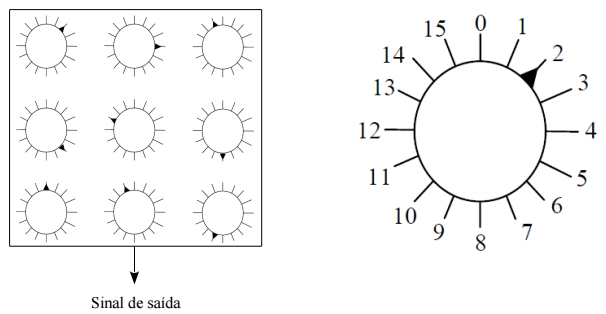
\includegraphics[scale=0.3]{problema.png}
		\end{figure}
	\end{frame}
	
	\begin{frame}
		\frametitle{Métodos}
		O trabalho foi implementado utilizando
		\begin{itemize}
			\item Python 2.7
			\begin{itemize}
				\item \textbf{Numpy}: programação utilizando \textit{arrays};
				\item \textbf{matplotlib}: plotagem dos gráficos;
				\item \textbf{scipy}: testes estatísticos.\\[1cm]
			\end{itemize}
		\end{itemize}
		
		Obs: Para cada teste, o algoritmo genético foi executado \textbf{100} vezes.
	\end{frame}
	
	\begin{frame}
		\frametitle{Resultados}
		\framesubtitle{Teste 1}
		\textbf{Cruzamento uniforme VS. 1 ponto de corte}
		\begin{figure}[H]
			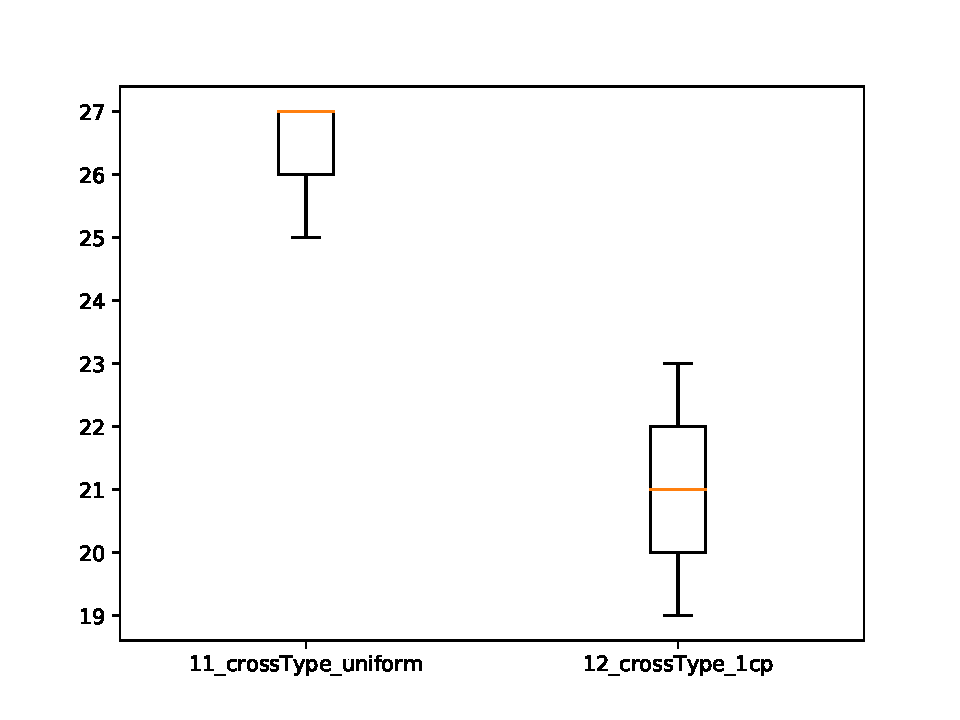
\includegraphics[scale=0.5]{../relatorio/teste1.pdf}
		\end{figure}
	\end{frame}
	
	\begin{frame}
		\frametitle{Resultados}
		\framesubtitle{Teste 2}
		\textbf{Seleção por torneio VS. roleta}
		\begin{figure}[H]
			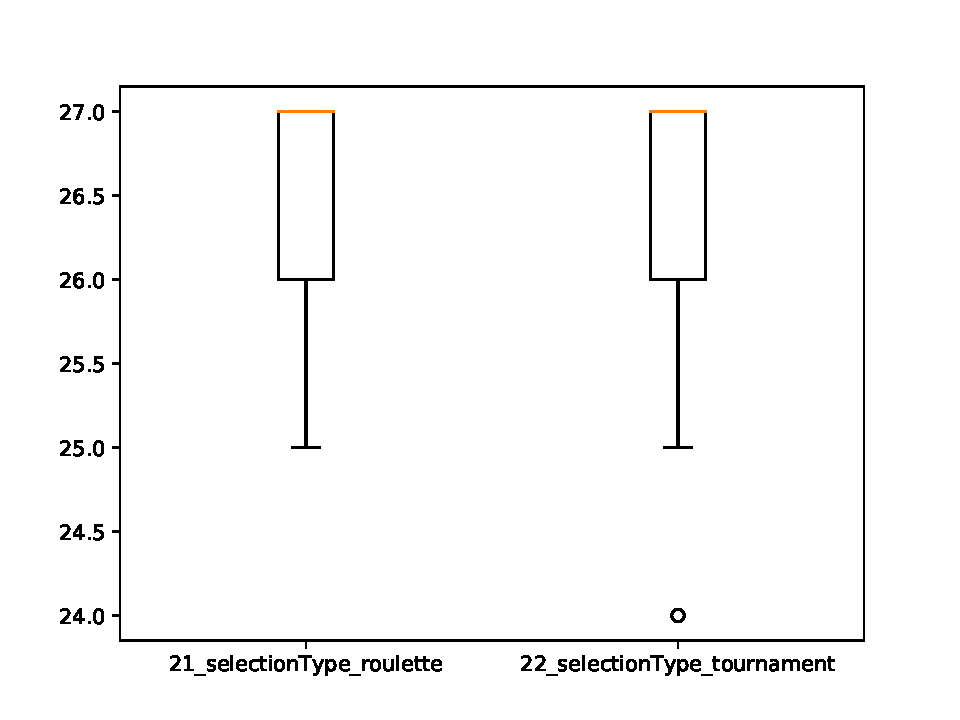
\includegraphics[scale=0.5]{../relatorio/teste2.pdf}
		\end{figure}
	\end{frame}
	
	\begin{frame}
		\frametitle{Resultados}
		\framesubtitle{Teste 3}
		\textbf{Mutação bit-a-bit VS. escolha aleatória de bit}
		\begin{figure}[H]
			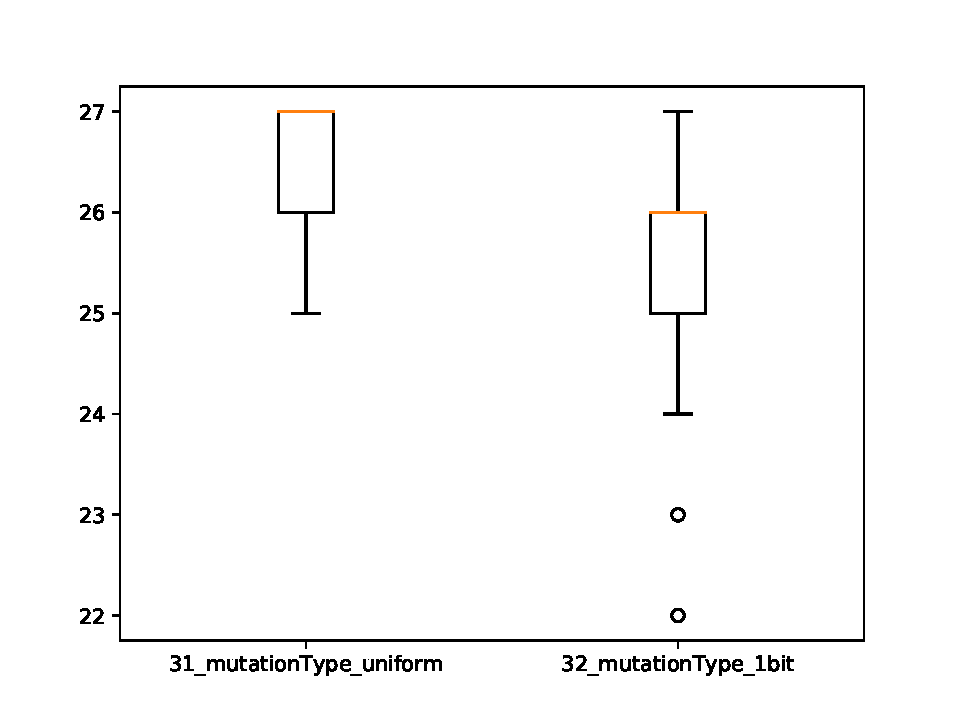
\includegraphics[scale=0.5]{../relatorio/teste3.pdf}
		\end{figure}
	\end{frame}
	
	\begin{frame}
		\frametitle{Resultados}
		\framesubtitle{Teste 4}
		\textbf{Probabilidades de cruzamento iguais a 0.2/0.5/0.8}
		\begin{figure}[H]
			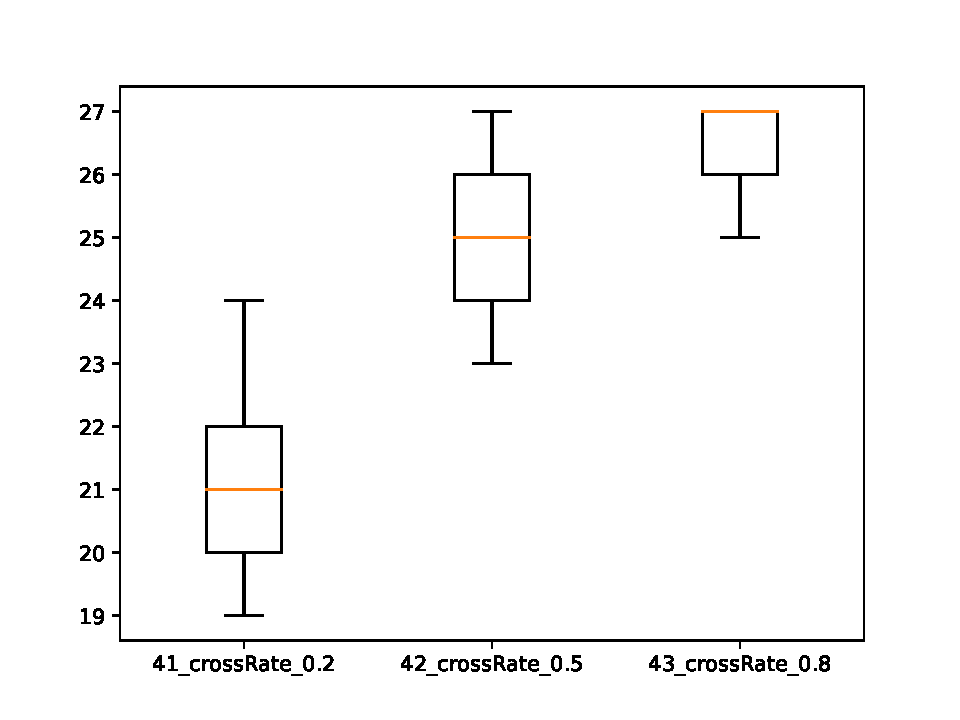
\includegraphics[scale=0.5]{../relatorio/teste4.pdf}
		\end{figure}
	\end{frame}
	
	\begin{frame}
		\frametitle{Resultados}
		\framesubtitle{Teste 4}
		\textbf{Probabilidades de mutação iguais a 0.025/0.05/0.1/0.5/0.75}
		\begin{figure}[H]
			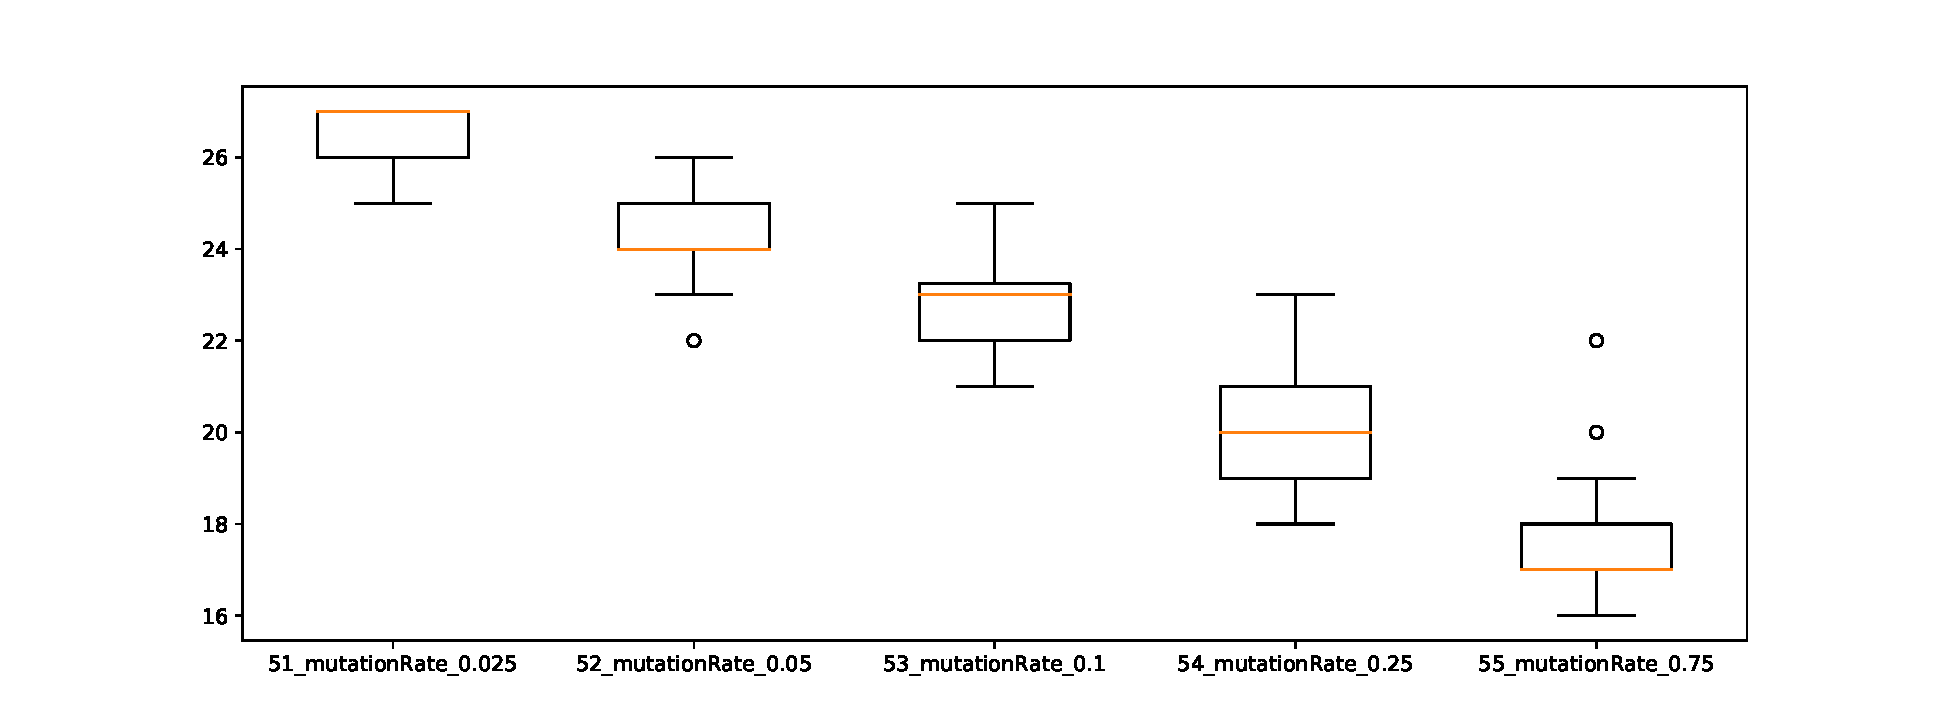
\includegraphics[scale=0.35]{../relatorio/teste5.pdf}
		\end{figure}
	\end{frame}
	
	\begin{frame}
		\frametitle{Resultados}
		\framesubtitle{Avaliação final}
		Usando a configuração ótima encontrada, variou-se o número de gerações ($K$) e de indivíduos na população ($T$).
		
		\begin{figure}[!hb]
			\begin{subfigure}[b]{0.5\textwidth}
				\centering
				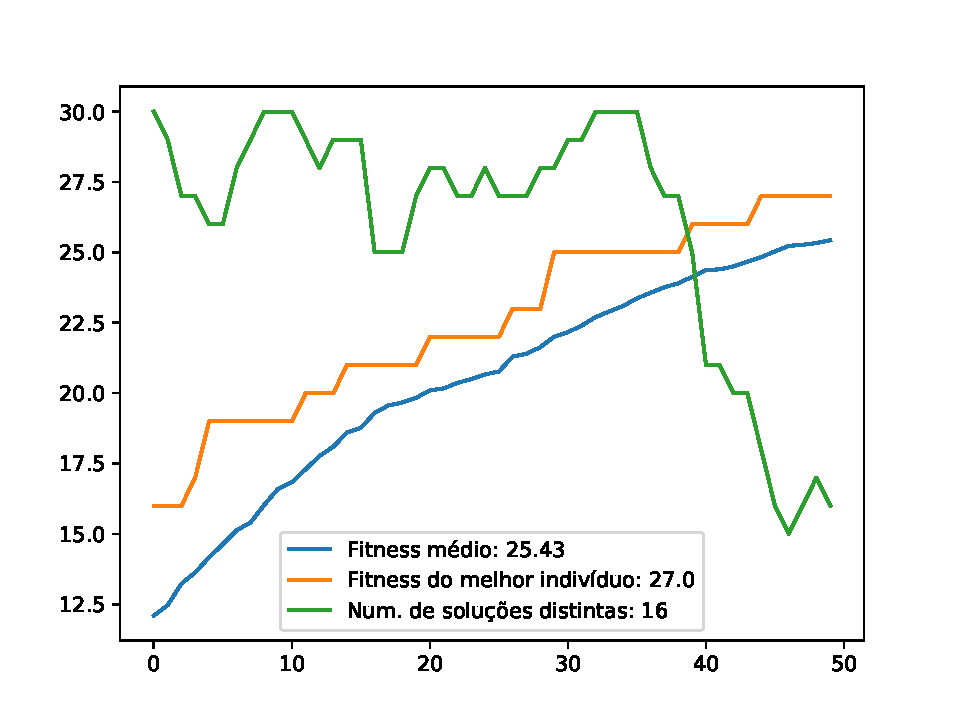
\includegraphics[width=\textwidth]{../relatorio/teste6_30_50.pdf}
				\caption{$(T,K)=(30,50)$}
			\end{subfigure}%
			\begin{subfigure}[b]{0.5\textwidth}
				\centering
				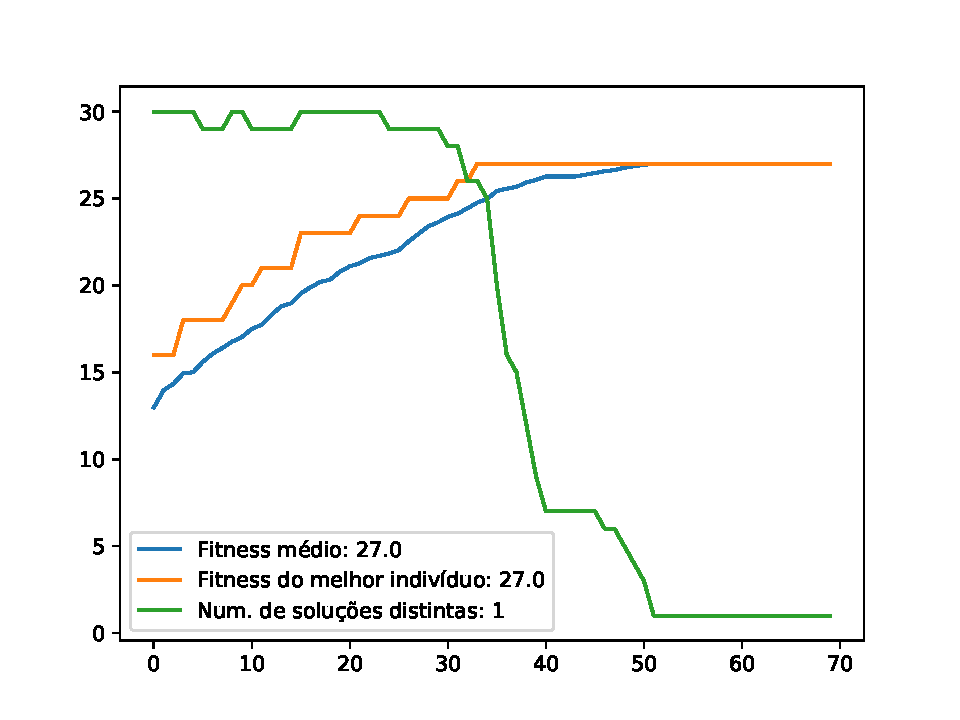
\includegraphics[width=\textwidth]{../relatorio/teste6_30_70.pdf}
				\caption{$(T,K)=(30,70)$}
			\end{subfigure}%
		\end{figure}
	\end{frame}
	
	\begin{frame}
		\frametitle{Resultados}
		\framesubtitle{Avaliação final}
		\begin{figure}[!hb]
			\begin{subfigure}[b]{0.5\textwidth}
				\centering
				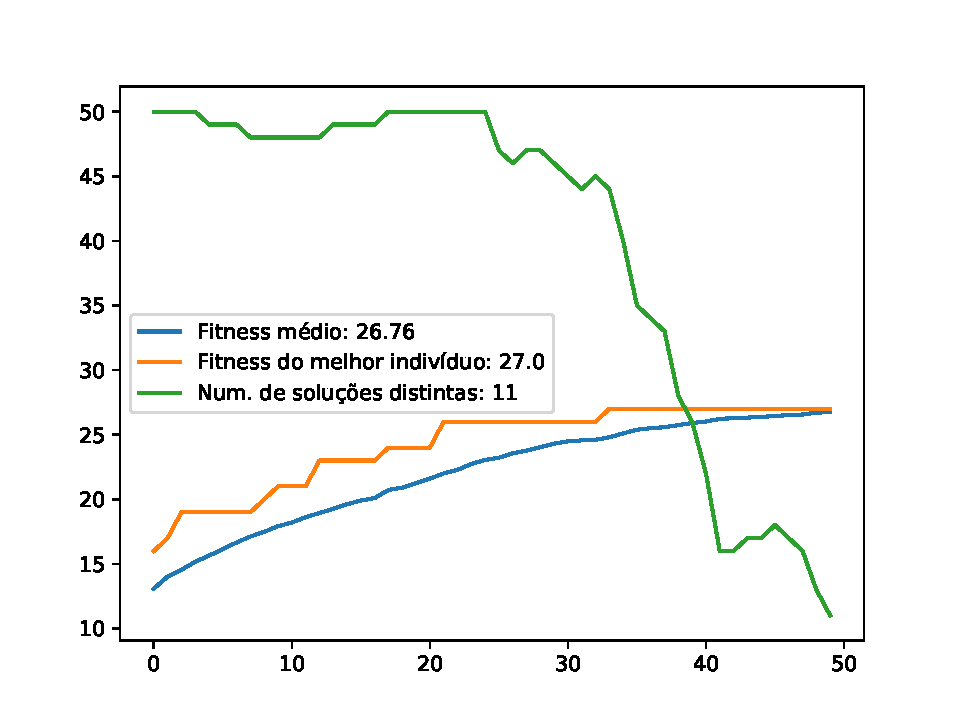
\includegraphics[width=\textwidth]{../relatorio/teste6_50_50.pdf}
				\caption{$(T,K)=(50,50)$}
			\end{subfigure}%
			\begin{subfigure}[b]{0.5\textwidth}
				\centering
				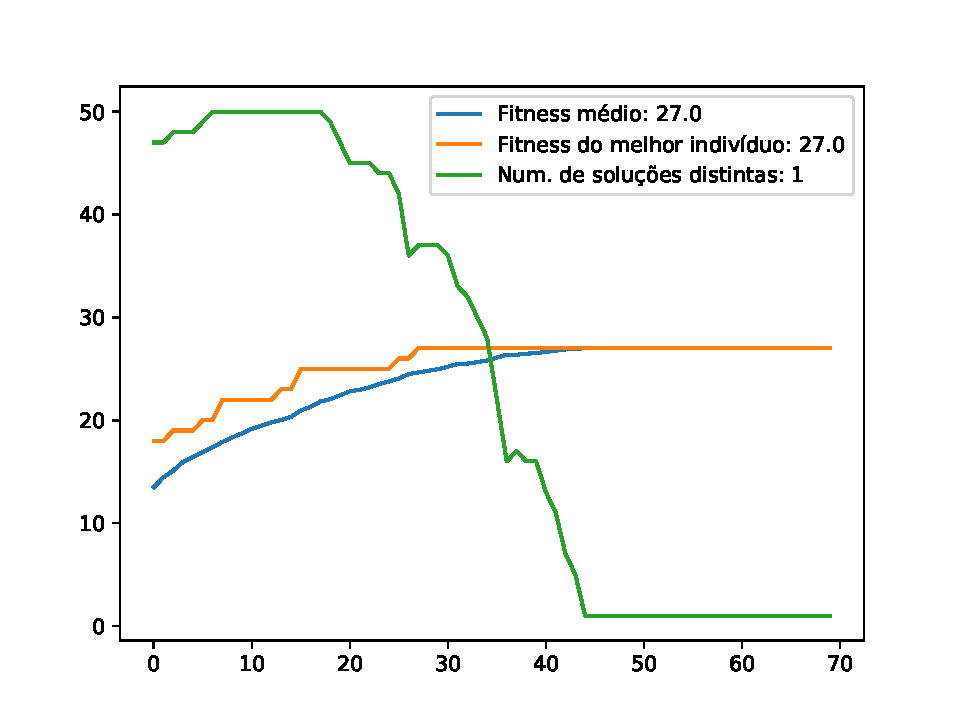
\includegraphics[width=\textwidth]{../relatorio/teste6_50_70.pdf}
				\caption{$(T,K)=(50,70)$}
			\end{subfigure}%
		\end{figure}
	\end{frame}
	
	\begin{frame}
		\begin{center}
			\textbf{\LARGE Obrigado!}
		\end{center}
	\end{frame}
\end{document}